% =============================================================
% P4 Firewall Poster (3 Pages, SIGCOMM Template)
% Compile on Overleaf with: pdflatex
% =============================================================

\documentclass[sigconf,nonacm]{acmart}

\settopmatter{printacmref=false}
\renewcommand\footnotetextcopyrightpermission[1]{}
\pagestyle{plain}

\acmConference{Project Poster}{April 2026}{Hyderabad, India}
\acmBooktitle{}
\acmDOI{}
\acmISBN{}

\usepackage{booktabs}
\usepackage{array}
\usepackage{amsmath}
\usepackage{graphicx}
\usepackage{tikz}
\usepackage{pgfplots}
\usepackage{float}
\pgfplotsset{compat=1.18}

\title{P4-Firewall+: Programmable Data-Plane Firewall with DNS DPI, Encrypted DNS Controls, and DNS Query-Rate Defense}

\author{Maloth Sravanthi}
\affiliation{%
  \institution{School of Computer and Information Sciences, University of Hyderabad}
  \country{India}
}
\author{Meher}
\affiliation{%
  \institution{School of Computer and Information Sciences, University of Hyderabad}
  \country{India}
}
\author{Indrashis Manna}
\affiliation{%
  \institution{School of Computer and Information Sciences, University of Hyderabad}
  \country{India}
}

\begin{document}
\maketitle
\twocolumn

% ========================= PAGE 1 =========================

\section*{Abstract}
This poster presents a completed programmable firewall implemented in P4 by
extending the p4lang/tutorials firewall baseline with DNS-aware controls and
stronger policy depth. The final system combines three active layers in one
switch pipeline: IP blacklist enforcement, DNS deep packet inspection (DPI), and
TCP stateful filtering using Bloom filters. The implementation includes
query-rate DNS defense logic, encrypted DNS controls for DoT and DoH-like
traffic classes, and 4-label DNS parsing support for richer domain matching.
Deployed on BMv2 with Mininet, the solution is validated through packet-level
tests, runtime counters, and table inspection.

\section*{Keywords}
P4, Programmable Data Plane, Firewall, DNS DPI, BMv2, Mininet, Stateful Filtering.

\section{Introduction}
Modern network defense requires fast decisions that combine flow state,
application-level context, and policy memory. CPU-centric inspection paths can
become a bottleneck under DNS-heavy loads, while simple packet filtering lacks
domain-level awareness. P4 allows protocol-aware parsing and policy enforcement
directly in the forwarding path.

This work delivers a complete firewall that merges TCP state tracking and
DNS-aware filtering in a single data-plane pipeline. The architecture is
operational, reproducible, and aligned with research-backed programmable data
plane security design.

\section{Literature Survey}
\textbf{P4 foundation.} Bosshart et al. introduced protocol-independent packet
processing and custom switch pipeline programming.

\textbf{Base GitHub firewall.} The p4lang/tutorials firewall exercise provides
stateful TCP admission control using Bloom-filter connection memory.

\textbf{DNS DPI in programmable data planes.} P4DDPI (NDSS MADWeb 2022)
demonstrates DNS parsing and policy enforcement inside the data plane.

\textbf{Our contribution path.} This project combines and extends these lines
into one integrated firewall with TCP stateful filtering, DNS DPI, IP policy
layers, encrypted DNS controls, query-rate defense, and deeper domain parsing.

% ========================= PAGE 2 =========================

\section{Problem Statement}
The baseline GitHub firewall is effective for TCP statefulness, but DNS-focused
security needs additional in-pipeline controls:
\begin{itemize}
  \item domain-level DNS query filtering,
  \item destination-IP policy integration,
  \item encrypted DNS endpoint controls,
  \item repeated DNS query burst defense,
  \item deeper domain parsing depth for richer policy keys.
\end{itemize}

The goal is a unified P4 firewall with these capabilities delivered in one
runnable architecture.

For TCP flow memory behavior, Bloom-filter false-positive probability follows:
\begin{equation}
  p = \left(1 - e^{-kn/m}\right)^k
\end{equation}
where $m$ is the Bloom-array size, $k$ is number of hashes, and $n$ is inserted
flow keys.

\section{Modifications to existing GitHub project}
The modified firewall extends the base implementation with the following
completed upgrades:
\begin{enumerate}
  \item UDP and DNS parser integration in the main firewall pipeline.
  \item DNS domain parsing expanded to 4 labels.
  \item \texttt{domain\_filter} expanded to 4-key matching:
  \texttt{(label1\_len, label2\_len, label3\_len, label4\_len)}.
  \item Static \texttt{ip\_blacklist} and register-backed IP control logic.
  \item DNS query-rate defense with threshold-triggered drop behavior.
  \item Encrypted DNS endpoint control table with DoT/DoH-like counters.
  \item Controller support for 3-label and 4-label domain key generation.
  \item Standalone build/run and runtime load workflow for reproducible testing.
\end{enumerate}

\section{Experimental Setup \& Test Bed}
\textbf{Platform:} Linux/P4 VM environment with p4c, BMv2
\texttt{simple\_switch\_grpc}, Mininet, and Scapy test utilities.

\textbf{Topology:} 4-host, 4-switch pod topology. Switch \texttt{s1} runs
\texttt{firewall.p4}; \texttt{s2}, \texttt{s3}, and \texttt{s4} run
\texttt{basic.p4}.

\textbf{Validation flow:} ping connectivity checks, blocked-domain DNS tests,
allowed-domain DNS tests, multi-domain blacklist checks, and runtime
counter/table verification.

\textbf{Observed behavior:} blocked malicious DNS requests do not reach receiver
endpoints, legitimate DNS requests are forwarded, and switch register/table
state confirms runtime enforcement.

% ========================= PAGE 3 =========================

\section{Comparison: GitHub vs Modified version (Graph/Table)}

\begin{table}[H]
\caption{Capability-level comparison between baseline and modified firewall.}
\label{tab:capability}
\centering
\small
\begin{tabular}{>{\raggedright\arraybackslash}p{0.62\textwidth}cc}
\toprule
\textbf{Capability} & \textbf{GitHub Base} & \textbf{Modified} \\
\midrule
Stateful TCP Bloom-filter firewall & Yes & Yes \\
DNS parser and DPI path & No & Yes \\
Domain blacklist enforcement & No & Yes \\
Static IP blacklist enforcement & No & Yes \\
Register-backed IP control behavior & No & Yes \\
DNS query-rate defense behavior & No & Yes \\
Encrypted DNS endpoint controls & No & Yes \\
4-label domain parsing and matching & No & Yes \\
\bottomrule
\end{tabular}
\end{table}

\begin{figure}[H]
\centering
\begin{tikzpicture}
\begin{axis}[
    ybar,
    bar width=18pt,
    width=0.70\textwidth,
    height=0.38\textheight,
    ymin=0,
    ymax=8,
    ylabel={Implemented Capabilities},
    symbolic x coords={GitHub Base,Modified},
    xtick=data,
    nodes near coords,
    nodes near coords align={vertical},
    ymajorgrids=true,
    grid style=dashed,
    enlarge x limits=0.40
]
\addplot coordinates {(GitHub Base,1) (Modified,8)};
\end{axis}
\end{tikzpicture}
\caption{Security capability coverage count (out of 8 capabilities).}
\label{fig:coverage}
\end{figure}

\section{Conclusion}
The final firewall design delivers a clear capability expansion over the base
GitHub version by integrating transport-layer statefulness and DNS-aware policy
intelligence in one programmable data-plane implementation. The architecture
combines IP policy enforcement, DNS parsing and filtering, encrypted DNS controls,
and query-rate defense with practical runtime observability through counters and
tables.

This completed implementation demonstrates the effectiveness of P4-based security
pipelines for modern network defense and provides a strong, reproducible platform
for academic demonstration and extension.

\section*{References}
\begin{enumerate}
  \item Bosshart et al., \textit{P4: Programming Protocol-Independent Packet Processors}, ACM SIGCOMM CCR, 2014.
  \item p4lang/tutorials, \textit{Firewall Exercise}, GitHub repository.
  \item AlSabeh et al., \textit{P4DDPI: Securing P4-Programmable Data Plane Networks via DNS Deep Packet Inspection}, MADWeb at NDSS, 2022.
  \item BMv2 behavioral model documentation.
  \item Mininet documentation.
\end{enumerate}

\end{document}
